% This is samplepaper.tex, a sample chapter demonstrating the
% LLNCS macro package for Springer Computer Science proceedings;
% Version 2.20 of 2017/10/04
%
\documentclass[runningheads]{llncs}
%
\usepackage{graphicx}
\usepackage{enumitem}
\usepackage{url}
\usepackage{float}
\usepackage{amsmath,amsfonts,amssymb}
\renewcommand{\labelitemii}{$\cdot$}
\renewcommand\labelitemi{\raisebox{0.4ex}{\tiny$\bullet$}}
% Used for displaying a sample figure. If possible, figure files should
% be included in EPS format.
%
% If you use the hyperref package, please uncomment the following line
% to display URLs in blue roman font according to Springer's eBook style:
% \renewcommand\UrlFont{\color{blue}\rmfamily}

\begin{document}
%
\title{Meltdown Security Vulnerability\\
{\large CS305/341 Course -- Project Report}}
%
%\titlerunning{Abbreviated paper title}
% If the paper title is too long for the running head, you can set
% an abbreviated paper title here
%
\author{Vamsi Krishna Reddy Satti \and
Vighnesh Reddy Konda \and
\\Niranjan Vaddi \and
Sai Praneeth Reddy Sunkesula}
%
\authorrunning{Vamsi, Vighnesh, Niranjan, Praneeth}
% First names are abbreviated in the running head.
% If there are more than two authors, 'et al.' is used.
%
\institute{Department of Computer Science and Engineering,\\
Indian Institute of Technology Bombay, Mumbai, India\\
\email{\{160050064, 160050090, 160050099, 160050100\}@iitb.ac.in}}\\
%
\titlerunning{Meltdown Security Vulnerability}
\maketitle              % typeset the header of the contribution
%
\begin{abstract}
A central security feature of today's operating systems is memory isolation. Operating systems ensure that user programs cannot access each other’s memory or kernel memory. This isolation is a cornerstone of our computing environments and allows running multiple applications at the same time on personal devices or executing processes of multiple users on a single machine in the cloud.
Out-of-order execution  is  an  indispensable  performance  feature  and present in a wide range of modern processors. Meltdown exploits side effects of out-of-order execution on modern processors to read arbitrary kernel-memory locations including personal data  and passwords. Meltdown enables an adversary to read memory of other processes or virtual machines in the cloud without any permissions or privileges, affecting millions of customers and virtually every user of a personal computer
In this project we explored the mechanism of Meltdown, plausible solutions and a Proof of Concept that demonstrates how a program can read data from a given kernel virtual address.

\keywords{Meltdown  \and Side channel \and Cache \and Flush+Reload \and Out-of-order execution}
\end{abstract}
%
%
%
\section{Background}
\subsection{The Memory Subsystem}
To isolate processes from each other, CPUs support virtual address spaces where virtual addresses are translated to physical addresses. Each process can only reference data that belongs to its own virtual address space. Each virtual address space itself is split into a user and a kernel part. The isolation between the kernel and user processes is typically realized by a supervisor bit of the processor that defines whether a memory page of the kernel can be accessed or not.  This hardware feature allows operating systems to map the kernel into the address space of every process and to have very efficient transitions from the user process to the kernel. In effect, the address space of every process includes the entire user space, as well as the entire kernel space, which typically also has all physical memory (in use) mapped. On Linux and OS X, this is done via a direct-physical map, i.e., the entire physical memory is directly mapped to a pre-defined virtual address

\subsection{Out of Order Execution and Cache}
Out-of-order vulnerable CPUs allow an unprivileged process to load data from a privileged (kernel or physical) address into a temporary CPU register. Moreover, the CPU even performs further computations based on this register value, e.g., access to an array based on the register value. The processor ensures correct program execution, by simply discarding the results of the memory lookups (e.g., the modified register states), if it turns out that an instruction should not have been executed. Hence, on the architectural level (e.g., the abstract definition of how the processor should perform computations), no security problem arises. 

Tomasulo developed an algorithm that enabled dynamic scheduling of instructions to allow out-of-order execution. This algorithm uses Unified Reservation stations that permit the CPU to fetch and re-use a data value as soon as it has been computed, rather than waiting for it to be stored in a register and re-read. To realize this, instructions are issued in sequence to Reservation Stations which buffer the instruction as well as the operands of the instruction. If the operand is not available, the Reservation Station listens on a Common Data Bus (CDB) for the operand to become available. When the operand becomes available, the Reservation Station buffers it, and the execution of the instruction can begin. Functional Units (such as an adder or a multiplier), each have their own corresponding Reservation Station. The output of the Functional Unit connects to the Common Data Bus, where Reservation Stations are listening for the operands they need.

Tomasulo's Algorithm uses register renaming to correctly perform out-of-order execution. Register renaming is a technique that eliminates the false data dependencies arising from the reuse of architectural registers by successive instructions that do not have any real data dependencies between them. The elimination of these false data dependencies reveals more instruction-level parallelism in an instruction stream. 

On the Intel architecture, the pipeline consists of the front-end, the execution engine (back-end) and the memory subsystem. x86 instructions are fetched by the front-end from the memory and decoded to micro-operations ($\mu$OPs) which are continuously sent to the execution engine. The Reorder Buffer is responsible for register allocation, register renaming and retiring. Additionally, other optimizations like move elimination or the recognition of zeroing idioms are directly handled by the reorder buffer. The μOPs are forwarded to the Unified Reservation Station that queues the operations on exit ports that are connected to Execution Units. Each execution unit can perform different tasks like ALU operations, AES operations, address generation units (AGU) or memory loads and stores. AGUs as well as the load and store execution units are directly connected to the memory subsystem to process its requests.

\section{What is Meltdown?}
Meltdown is a novel attack that allows overcoming memory isolation completely by providing a simple way for any user process to read the entire kernel memory of the machine it executes on, including all physical memory mapped in the kernel region. Meltdown does not exploit any software vulnerability, i.e., it works on all major operating systems. Instead, Meltdown exploits side-channel information available on most modern processors. Meltdown allows an adversary who can run code on the vulnerable processor to obtain a dump of the entire kernel address space, including any mapped physical memory. The root cause of the simplicity and strength of Meltdown are side effects caused by out-of-order execution.

Although the instructions executed out of order do not have any visible architectural effect on registers or memory, they have microarchitectural side effects. During the out-of-order execution, the referenced memory is fetched into a register and is also stored in the cache. If the out-of-order execution has to be discarded, the register and memory contents are never committed. Nevertheless, the cached memory contents are kept in the cache. We can leverage a microarchitectural side-channel attack such as Flush+Reload, which detects whether a specific memory location is cached, to make this microarchitectural state visible.
	
Meltdown exploits a race condition between memory access and privilege checking during instruction processing. Additionally, combined with a cache side-channel attack, this vulnerability allows a process to bypass the normal privilege checks that isolate the exploit process from accessing data belonging to the operating system and other running processes. The vulnerability allows an unauthorized process to read data from any address that is mapped to the current process's memory space. Since instruction pipelining is in the affected processors, the data from an unauthorized address will almost always be temporarily loaded into the CPU's cache during out-of-order execution —from which the data can be recovered. This can occur even if the original read instruction fails due to privilege checking, and/or if it never produces a readable result.

\section{Building Blocks of the Attack}
\subsection{Executing Transient Instructions}
The first building block of Meltdown is to make the CPU execute one or more instructions that would never occur in the executed path. An instruction, which is executed out of order, leaving measurable side effects, a transient instruction. Transient instructions introduce an exploitable side channel if their operation depends on a secret value. Accessing user-inaccessible pages, such as kernel pages, triggers an exception which generally terminates the application. If the attacker targets a secret at a user-inaccessible address, the attacker has to cope with this exception. There are two approaches:  exception handling and exception suppression.

With \textbf{exception handling}, we catch the exception effectively occurring after executing the transient instruction sequence, \textit{e.g.}  fork-and-crash, the attacking process forks, and the child accesses invalid memory and executes the transient instruction sequence before crashing. The parent process can then recover the secret by observing the microarchitectural state, e.g., through a side-channel and with exception suppression, we prevent the exception from occurring at all and instead redirect the control flow after executing the transient instruction sequence. Another approach is to install a signal handler that will be executed if a certain exception occurs, in this specific case a segmentation fault. This allows the attacker to issue the instruction sequence and prevent the application from crashing, reducing the overhead as no new process has to be created

In \textbf{exception suppression}, exceptions are prevented from being raised in the first place. \textit{e.g.} Transactional memory allows to group memory accesses into one seemingly atomic operation, (\textit{e.g.} Intel TSX) giving the option to roll-back to a previous state if an error occurs. Another approach is to use branch misprediction. Invalid memory access is put within a speculative instruction sequence that is only executed if a prior branch condition evaluates to true. By making sure that the condition never evaluates to true in the executed code path, we can suppress the occurring exception as the memory access is only executed speculatively. This technique may require a sophisticated training of the branch predictor.

\subsection{Building a Covert Channel}
The second building block of Meltdown is the transfer of the microarchitectural state, which was changed by the transient instruction sequence, into an architectural state. The transient instruction sequence can be seen as the sending end of a microarchitectural covert channel. The receiving end of the covert channel receives the microarchitectural state change and deduces the secret from the state.

Flush+Reload allows us to build a fast and low-noise covert channel. Depending on the secret value, the transient instruction sequence performs a regular memory access. After the transient instruction sequence accessed an accessible address, i.e., this is the sender of the covert channel; the address is cached for subsequent accesses. The receiver can then monitor whether the address has been loaded into the cache by measuring the access time to the address. Thus, the sender can transmit a ‘1’-bit by accessing an address which is loaded into the monitored cache, and a ‘0’-bit by not accessing such an address.

\section{Mitigations}
\subsection{Hardware Fixes}
As Meltdown exploits out-of-order execution, a trivial countermeasure would be to completely disable out-of-order execution. However, the performance impacts would be devastating, as the parallelism of modern CPUs could not be leveraged anymore. Thus, this is not a viable solution.
Meltdown is some form of race condition between the fetch of a memory address and the corresponding permission check for this address. Serializing the permission check and the register fetch can prevent Meltdown, as the memory address is never fetched if the permission check fails. However, this involves a significant overhead to every memory fetch, as the memory fetch has to stall until the permission check is completed.
A more plausible solution would be to introduce a hard split of user space and kernel space. This could be enabled optionally by modern kernels using a new hard split bit in a CPU control register. If the hard split bit is set, the kernel has to reside in the upper half of the virtual address space, and the user space has to reside in the lower half of the virtual address space. With this hard split, a memory fetch can immediately identify whether such a fetch of the destination would violate a security boundary, as the privilege level can be directly derived from the virtual address without any further lookups. The performance impacts of such a solution to be minimal. Furthermore, the backward compatibility is ensured, since the hard-split bit is not set by default and the kernel only sets it if it supports the hard-split feature.

\subsection{Software Patches}
\subsubsection{Kernel Address Space Layout Randomization (KASLR)}

Modern operating system kernels employ address space layout randomization (ASLR) to prevent control-flow hijacking attacks and code-injection attacks. While kernel security relies fundamentally on preventing access to address information, recent attacks have shown that the hardware directly leaks this information. Strictly splitting kernel space and user space has recently been proposed as a theoretical concept to close these side channels. However, this is not trivially possible due to architectural restrictions of the x86 platform.

\begin{figure}
\centerline{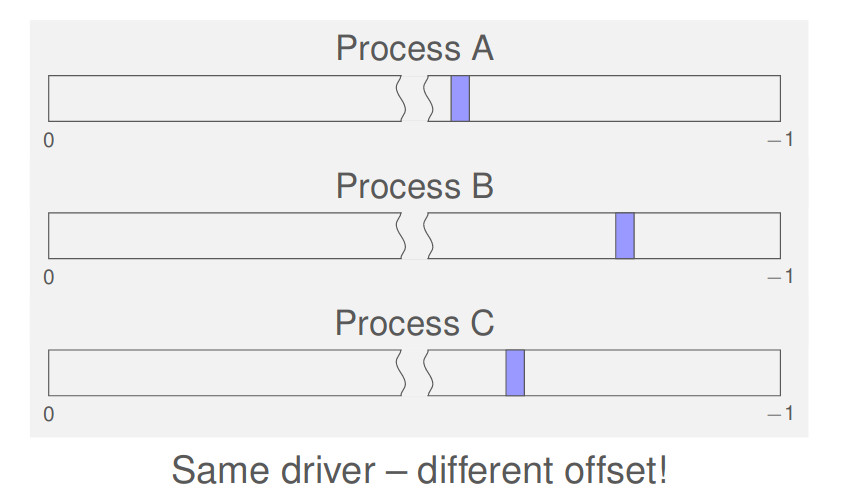
\includegraphics[scale=0.3]{images/kaslr.png}}
\caption{KASLR} \label{kaslr}
\end{figure}

Address space layout randomization (ASLR) can be used to make some kernel addresses or even all kernel addresses unpredictable for an attacker. Knowledge of virtual or physical address information can be exploited to bypass KASLR. Side-channel attacks (\textit{e.g.} attacks exploiting software prefetch instructions, Intel TSX, double page faults) targeting the page translation caches provide information about virtual and physical addresses to the user space.

\paragraph{Attacks exploiting double page faults}: If the memory location is valid, regardless of whether it is accessible or not, address translation table entries are copied into the corresponding address translation caches. The attacker then tries to access the same inaccessible memory location again. If the memory location is valid, the address translation is already cached and the page fault interrupt will take less time.  Thus, the attacker learns whether a memory location is valid or not, even if it is not accessible from the user space.

\paragraph{Attacks exploiting Intel TSX}: Double page faults can be exploited in combination with Intel TSX. But the timing differences are significantly less noisy. In this attack, the attacker again learns whether a memory location is valid, even if it is not accessible from the user space

\paragraph{Software prefetch instructions to trigger address translation}: The execution time of the prefetch instruction depends on which address translation caches hold the right translation entries. Thus, in addition to learning whether an inaccessible address is valid or not, an attacker learns its corresponding page size as well. If the attacker prefetches an inaccessible address in this kernel physical direct map corresponding to a user-accessible address, it will also be cached when accessed through the user address. Thus, the attacker can retrieve the exact physical address for any virtual address.

All the above attacks have in common that they exploit that the kernel address space is mapped in user space as well, and that accesses are only prevented through the permission bits in the address translation tables. Thus, they use the same entries in the paging structure caches.

With KASLR the direct-physical map offset is randomized, thus the attacker is required to obtain the randomized offset before mounting the Meltdown attack. If the attacker can successfully obtain a value from a tested address, the attacker can proceed to dump the entire memory from that location. This allows mounting Meltdown on a system despite being protected by KASLR within seconds.

\subsubsection{Kernel Address Isolation to have Side-channels Efficiently Removed (KAISER)}
The idea of Stronger Kernel  Isolation is to unmap kernel pages while the user process is in user space and switch to a separated kernel address space when entering the kernel. Consequently, user pages are not mapped in kernel space and only a minimal number of pages is mapped both in user space and kernel space. While this would prevent all microarchitectural attacks on kernel address space information on recent systems, it is not possible to implement Stronger Kernel Isolation without rewriting large parts of today’s kernels.
	
KAISER uses a shadow address space paging structure to separate kernel space and user space. The lower half of the shadow address space is synchronized between both paging structures. KAISER reduces the number of overlapping pages between user and kernel address space to the absolute minimum required to run on modern x86 systems. KAISER enforces a strict kernel and user space isolation such that the hardware does not hold any information about kernel addresses while running user processes.

\begin{figure}[H]
\centerline{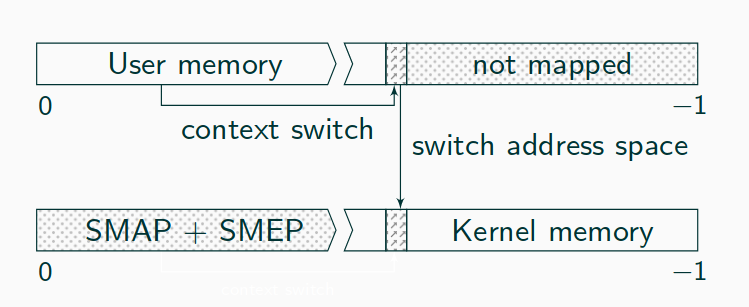
\includegraphics[scale=0.45]{images/kaiser.png}}
\caption{Shadow address space and Kernel Address Space - KAISER} \label{kaiser}
\end{figure}

Every process has two address spaces. One address space which has the user space mapped but not the kernel (i.e., the shadow address space), and a second address space which has the kernel mapped but the user space protected with SMAP and SMEP. SMEP protects against executing user space code in kernel mode. Any memory location that is user-accessible cannot be executed by the kernel. SMAP protects against invalid user memory references in kernel mode.
	
The main side-channel defense in KAISER is based on the separate shadow address spaces. This inadvertently protects from Meltdown attack as well. The invalid memory access instruction in Meltdown will not be able to load data from the inaccessible kernel address and thereby the transient instructions do not succeed. KAISER successfully eliminates the leakage.
	
As the two shadow address spaces have different CR3 register values, KAISER requires a CR3 update upon every context switch (user space to user space or user space to kernel space). The defined behavior of current Intel x86 processors is to perform implicit TLB flushes upon every CR3 update. An optimization is to tag the TLB entries with the CR3 register to avoid frequent TLB flushes due to switches between processes or between user mode and kernel mode. Intel x86 processors have such optimizations already implemented. KAISER benefits from these optimizations implicitly and consequently, its TLB management is efficient. KAISER has a low memory overhead of approximately 8 kB per user thread and a low runtime overhead of only 0.28\%.

\section{Our Proof of Concept Experiment}
\subsection{Reading the Secret}
To load data from the main memory into a register, the data in the main memory is referenced using a virtual address. In parallel to translating a virtual address into a physical address, the CPU also checks the permission bits of the virtual address, i.e., whether this virtual address is user accessible or only accessible by the kernel. Modern operating systems always map the entire kernel into the virtual address space of every user process.

\begin{figure}[H]
\centerline{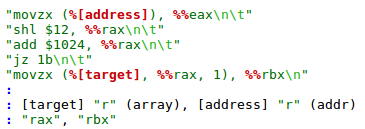
\includegraphics[scale=0.6]{images/asm_part.png}}
\caption{Assembly instructions for accessing the data from the location of secret \textbf{addr} and accessing the corresponding byte in probe array \textbf{array} to leak this secret} \label{asm_part}
\end{figure}

As a consequence, all kernel addresses lead to a valid physical address when translating them, and the CPU can access the content of such addresses. The only difference in accessing a user space address is that the CPU raises an exception as the current permission level does not allow to access such an address. Hence, the user space cannot simply read the contents of such an address. However, Meltdown exploits the out-of-order execution of modern CPUs, which still executes instructions in the small time window between the illegal memory access and the raising of the exception.

The last byte at the virtual address containing the secret is read into \texttt{rax} register using \texttt{movzx} instruction. This must raise an exception resulting in a segmentation fault when the instruction retires. However due to out-of-order execution, the next few instructions are executed transiently and their effect on the cache is not reverted. The segmentation fault raised is handled using a custom signal handler.\\

Signal Handling :
\begin{itemize}%%[itemsep = -0.75 mm, leftmargin=*]
\item \textit{Set up a signal handler}: We register a \texttt{SIGSEGV} signal handler \texttt{catch\_segv}, so when a \texttt{SIGSEGV} signal is raised, the handler function \texttt{catch\_segv} will be invoked.
\item \textit{Set up a checkpoint}: After the signal handler has finished processing the exception, it needs to let the program continue its execution from particular checkpoint. Therefore, we need to define a checkpoint first. This is achieved via \texttt{sigsetjmp(jbuf, 1)} which saves the stack context/environment in \texttt{jbuf} for later use by \texttt{siglongjmp()}.
\item \textit{Roll back to a checkpoint}: When \texttt{siglongjmp(jbuf, 1)} is called, the state saved in the \texttt{jbuf} variable is copied back in the processor and computation starts over from the return point of the \texttt{sigsetjmp()} function.
\end{itemize}

\begin{figure}[H]
\centerline{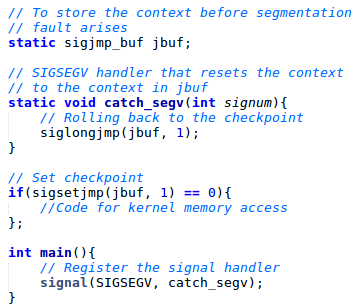
\includegraphics[scale=0.6]{images/allSig.png}}
\caption{Registering the custom signal handler; setting up the checkpoint and rolling back on segmentation fault} \label{seghandler}
\end{figure}

\subsection{Transmitting the secret}

\begin{figure}
\centerline{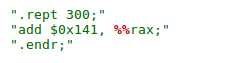
\includegraphics[scale=0.75]{images/rept.png}}
\caption{Filling the reorder buffer with dependent instructions} \label{rept}
\end{figure}

The transient instruction sequence is built in way to perform computations based on the secret which is stored in temporary registers before MOV instruction is retired. We utilize cache attacks that allow us to build fast and low-noise covert channel using the CPU’s cache. Thus, the transient instruction sequence has to encode the secret into the microarchitectural cache state. 

To achieve this, We allocate a probe array in memory and ensure that no part of this array is cached. To transmit the secret, the transient instruction sequence contains an indirect memory access to an address which is calculated based on the secret (inaccessible) value. The secret value stored in rax is multiplied by 4K and an offset of DELTA is added and this position in probe array is being accessed in the transient code. 

Since the transient instruction sequence races against raising the exception, reducing its runtime can significantly improve the performance of the attack. For instance, taking care that the address translation for the probe array is cached in the TLB increases the attack performance on some systems. 

To make sure the transient code executes before MOV retires, we fill the reorder buffer with dependent instructions which use a different execution unit than the ones we need. The dependency forces the CPU to execute one micro op at a time of the filling instructions. Using an execution unit different than the one we used in the leaking code make sure that the CPU can speculatively execute these while working on the fill pattern.

\subsection{Receiving the secret}

\begin{figure}[H]
\centerline{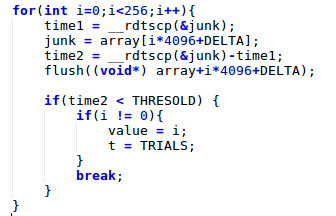
\includegraphics[scale=0.6]{images/getvalue.png}}
\caption{Accessing 256 addresses in probe array to deduce the secret at the receiver} \label{getvalue}
\end{figure}

In this step, we recover the secret value by leveraging a microarchitectural side-channel attack that transfers the cache state back into an architectural state. When the transient instruction sequence is executed, exactly one cache line of the probe array is cached. The position of the cached cache line within the probe array depends only on the secret which is read from kernel address space. Thus, the attacker iterates over all 256 pages of the probe array and measures the access time for every cache line at position DELTA on the page. The number of the page containing the cached cache line corresponds directly to the secret value.

\subsection{Results}
The secret program outputs the physical address of a secret string. Our program takes the physical address as the input and outputs the string starting from that location which actually belonged to the secret program.

\begin{figure}[H]
\centerline{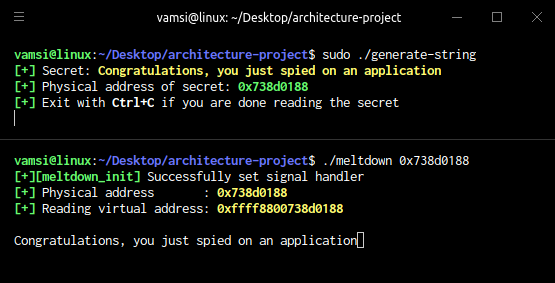
\includegraphics[scale=0.6]{images/secret.png}}
\caption{Meltdown attack to retrieve secret from another process} \label{getvalue}
\end{figure}

\section{Challenges}
\paragraph{The case of 0} If the exception is triggered while trying to read from an inaccessible kernel address, the register where the data should be stored, appears to be zeroed out. This is reasonable because if the exception is not handled, the user space application is terminated, and the value from the inaccessible kernel address could be observed in the register contents stored in the core dump of the crashed process. The direct solution to fix this problem is to zero out the corresponding registers. If the zeroing out of the register is faster than the execution of the subsequent instruction, the attacker may read a false value in the third step. To prevent the transient instruction sequence from continuing with a wrong value, i.e., ‘0’, Meltdown retries reading the address until it encounters a value different from ‘0’. As the transient instruction sequence terminates after the exception is raised, there is no cache access if the secret value is 0. Thus, Meltdown assumes that the secret value is indeed ‘0’ if there is no cache hit at all. 

But to increase the correctness of the secret value being read, we repeat Flush+Reload for TRAILS number of times and also repeat access to kernel address SUBTRAILS times in each trial. The loop breaks after receiving a non zero value. 

\paragraph{Access time computation}: Measuring the access times to probe an array must be done precisely, as these time intervals are very small. Moreover timing measurements would be inaccurate because of out-of-order execution if time is measured before the preceding instructions are completed. Hence, we have used pseudo-serialized instruction \texttt{rdtscp} for all the time calculations. 

\paragraph{Software Patches}: For our proof of concept experiment, we had to turn off KAISER, which was already patched to newer kernel versions (set pti=off in grub configurations). Even though Meltdown attack can be used to identify kernel physical offset while KASLR is turned on, in our proof of concept we turned it off so that the kernel offset is set to its default value.

\section{Contributions}

\begin{itemize}
    \item Vamsi Krishna \hfill     Linux Memory, KASLR, Meltdown, Code Optimizations\hspace{7pt}
    \item Vighnesh \hfill  KASLR, Meltdown, Linux Memory, PoC \hspace{7pt}
    \item Niranjan Vaddi\hfill  \hspace*{-7pt} KAISER, KASLR, Meltdown, PoC
    \item Sai Praneeth \hfill \hspace*{-7pt} KASLR, Meltdown, Linux Memory, PoC
\end{itemize}
% \begin{figure}
% \includegraphics[width=\textwidth]{fig1.eps}
% \caption{A figure caption is always placed below the illustration.
% Please note that short captions are centered, while long ones are
% justified by the macro package automatically.} \label{fig1}
% \end{figure}

%
% the environments 'definition', 'lemma', 'proposition', 'corollary',
% 'remark', and 'example' are defined in the LLNCS documentclass as well.
%

%
% ---- Bibliography ----
%
% BibTeX users should specify bibliography style 'splncs04'.
% References will then be sorted and formatted in the correct style.
%
\bibliographystyle{splncs04}
% \bibliography{mybibliography}
%
\begin{thebibliography}{8}
\bibitem{ref_meltdown}
Moritz Lipp et al.: Meltdown: Reading Kernel Memory from User Space. 27th {USENIX} Security Symposium ({USENIX} Security 18) (2018) \url{https://meltdownattack.com/meltdown.pdf}

\bibitem{ref_kaslr}
Gruss, D. et al.: KASLR is Dead: Long Live KASLR
\url{https://gruss.cc/files/kaiser.pdf}

\bibitem{ref_projectzero}
Jann Horn et al.: Google Project Zero
\url{https://googleprojectzero.blogspot.com/2018/01/reading-privileged-memory-with-side.html}

\bibitem{ref_wikilinuxpti}
Wikipedia contributors: Kernel page-table isolation
\url{https://en.wikipedia.org/wiki/Kernel_page-table_isolation}

\bibitem{ref_wikimeltdown}
Wikipedia contributors: Meltdown (security vulnerability)
\url{https://en.wikipedia.org/wiki/Meltdown_(security_vulnerability)}

\bibitem{ref_githubrepo}
Meltdown PoC Github
\url{https://github.com/IAIK/meltdown}

\bibitem{ref_kaslr_meltdown}
Gruss, D. et al.: How to have a Meltdown
\url{https://gruss.cc/files/cryptacus_training_2018.pdf}

\end{thebibliography}
\end{document}
